
\chapter{Metody vizualizace a porovnání}

Cílem této knihovny není pouze vizualizovat sekundární strukturu RNA, ale také
usnadnit analýzu rozdílů a podobností mezi více strukturami RNA. Proto jsme se
zaměřili na práci s radiálními diagramy.

Kromě toho jsme rozpoznali potenciál generování distribuce na základě vzorové
struktury, jak to dělá nástroj Traveler. Výstupem Traveleru je soubor ve
formátu JSON, který obsahuje informace o vzoru každého nukleotidu a provedených
úpravách.

V důsledku toho jsme se rozhodli používat v našich metodách zmíněné mapování na
referenční strukturu. Náš nástroj je tudíž schopný pracovat s $N$ strukturami,
mezi nimiž je referenční struktura, ze které jsou generovány všechny ostatní
struktury.

\section{Překládání struktur}

Vzhledem k tomu, že struktury odvozené od stejného vzoru jsou obvykle velmi
podobné, má smysl umožnit jejich překrytí, aby se spojily společné části a
zvýraznily se rozdíly. Pouhým přeložením podobných struktur přes sebe však
získáme výsledek, který neposkytuje příliš zajímavé informace a je málo
přehledný.

\begin{figure}[H]
  \centering
  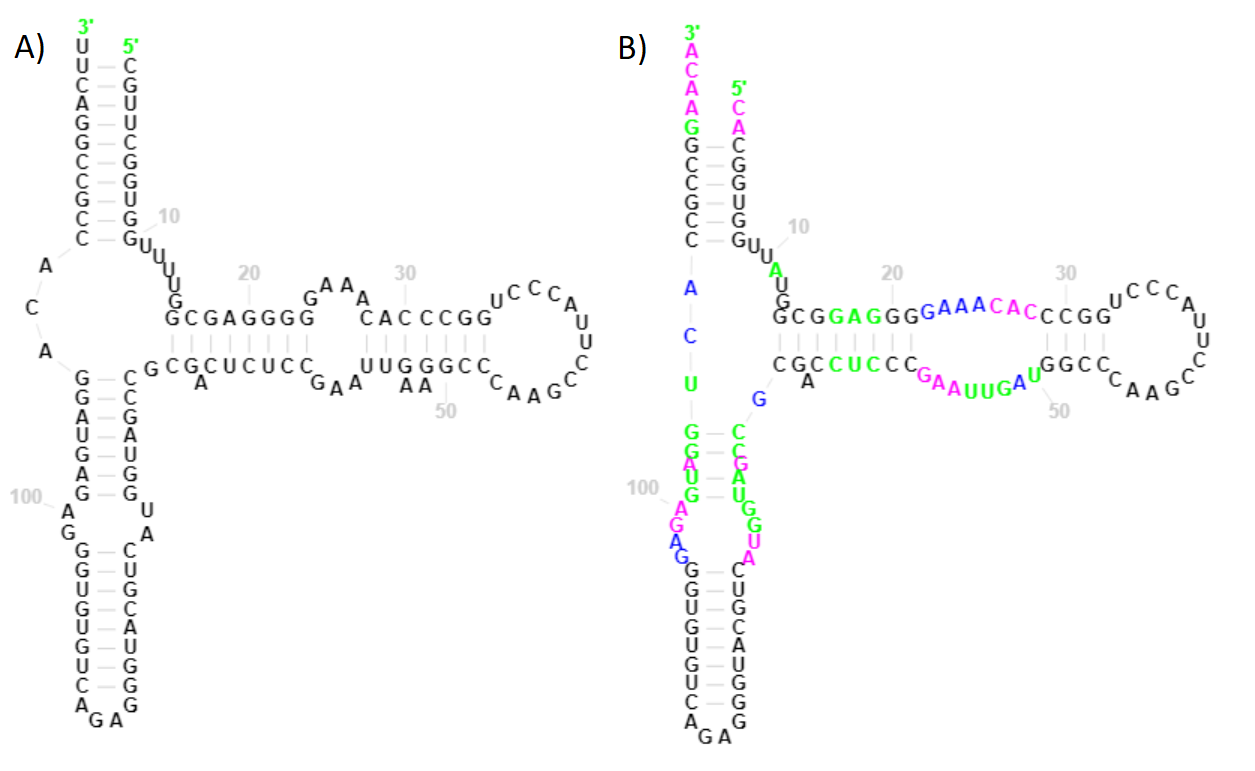
\includegraphics[width=140mm]{../img/kap02/align/structures.png}
  \caption{Struktury vedle sebe.}
\end{figure}

\begin{figure}[H]
  \centering
  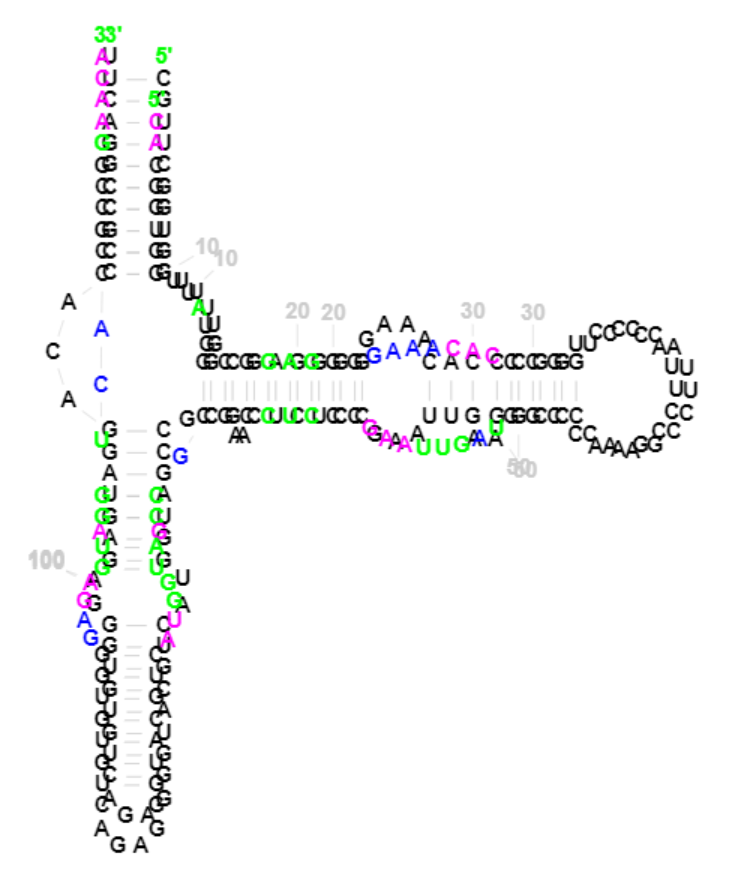
\includegraphics[height=90mm]{../img/kap02/align/unaligned.png}
  \caption{Struktury přeložené přes sebe.}
\end{figure}

Je potřeba najít způsob, jak řešit problém přesunu a zarovnání struktury,
protože manuální manipulace pomocí přetažení myší nebo zadávání pozice může být
zbytečně obtížná, zejména pokud se snažíme dosáhnout přesného zarovnání. Proto
je velmi užitečné umožnit zarovnání sekundární RNA struktury na konkrétní
nukleotid nebo skupinu nukleotidů ze vzorové struktury. 

Pokud je vybrán vzorový nukleotid $v$ pro určitý nukleotid $n$ z ostatních
struktur, je celá struktura přesunuta tak, aby se nukleotidy $v$ a $n$
překrývaly. Pokud se snažíme najít větší skupinu nukleotidů, na které chceme
strukturu zarovnat, koukáme se na posunutí pro konkrétní nukleotidy a následně
vybereme takové posunutí které zarovná nejvíc nukleotidů.

\begin{figure}[H]
  \centering
  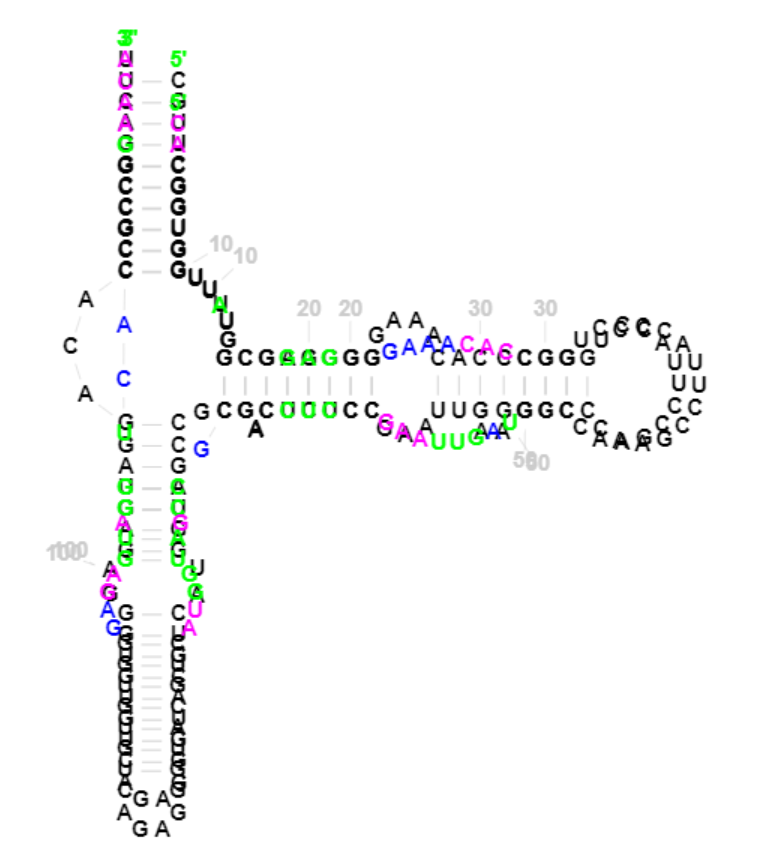
\includegraphics[height=90mm]{../img/kap02/align/alignedAlpha1.png}
  \caption{Struktury přeložené přes sebe a zarovnané.}
\end{figure}

Pouhým přeložením struktur nelze snadno rozeznat, které nukleotidy jsou
společné a překrývají se a které nejsou. Přidáním průhlednosti je možné tuto
situaci rozlišit, protože překrývající se nukleotidy budou mít sytější barvu
než ty, které se nepřekrývají.

\begin{figure}[H]
  \centering
  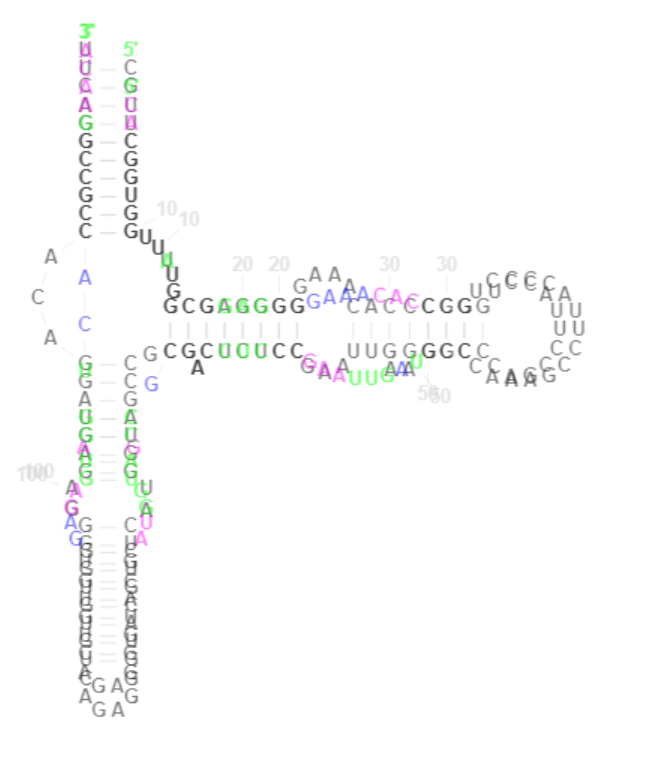
\includegraphics[height=90mm]{../img/kap02/align/aligned.png}
  \caption{Struktury přeložené přes sebe, zarovnané a s průhledností.}
\end{figure}

Zarovnávání struktur bohužel neřeší všechny výzvy. Výsledné obrázky se mohou
zdát rozmazané. To je způsobeno tím, že ačkoli má nukleotid vzorový nukleotid,
který je stejný, jeho pozice se může v rozložení mírně lišit v důsledku metody
generování dat. Tento fakt může způsobit, že popisky nukleotidů vypadají
rozmazaně.

Jako přímočaré řešení se může zdát posunout jednotlivé nukleotidy, které jsou
blízko sebe, aby dokonale překrývaly jejich vzory. Věříme, že by to vyřešilo
zmíněný problém. Nicméně naše knihovna tuto funkci přímo neimplementuje.

\section{Transformace na vzor}

Užitečnou metodou je transformace mezi vzorovou a cílovou strukturou. Každý
nukleotid, který má svůj vzorový nukleotid, se přemístí na pozici vzorového
nukleotidu a nukleotidy, které ve vzoru nejsou, jsou skryté. Tato metoda je
velmi užitečná pro práci s dvěma strukturami, které jsou si podobné, nebo pro
získání počátečního přehledu o tom, co je na co namapováno. Slabou stránkou
této metody je její použití při práci s více než dvěma strukturami nebo
strukturami, které jsou velmi odlišné. V takových situacích se na obrazovce
děje mnoho věcí a je obtížné se soustředit a vypozorovat něco užitečného.

\begin{figure}[H]
  \centering
  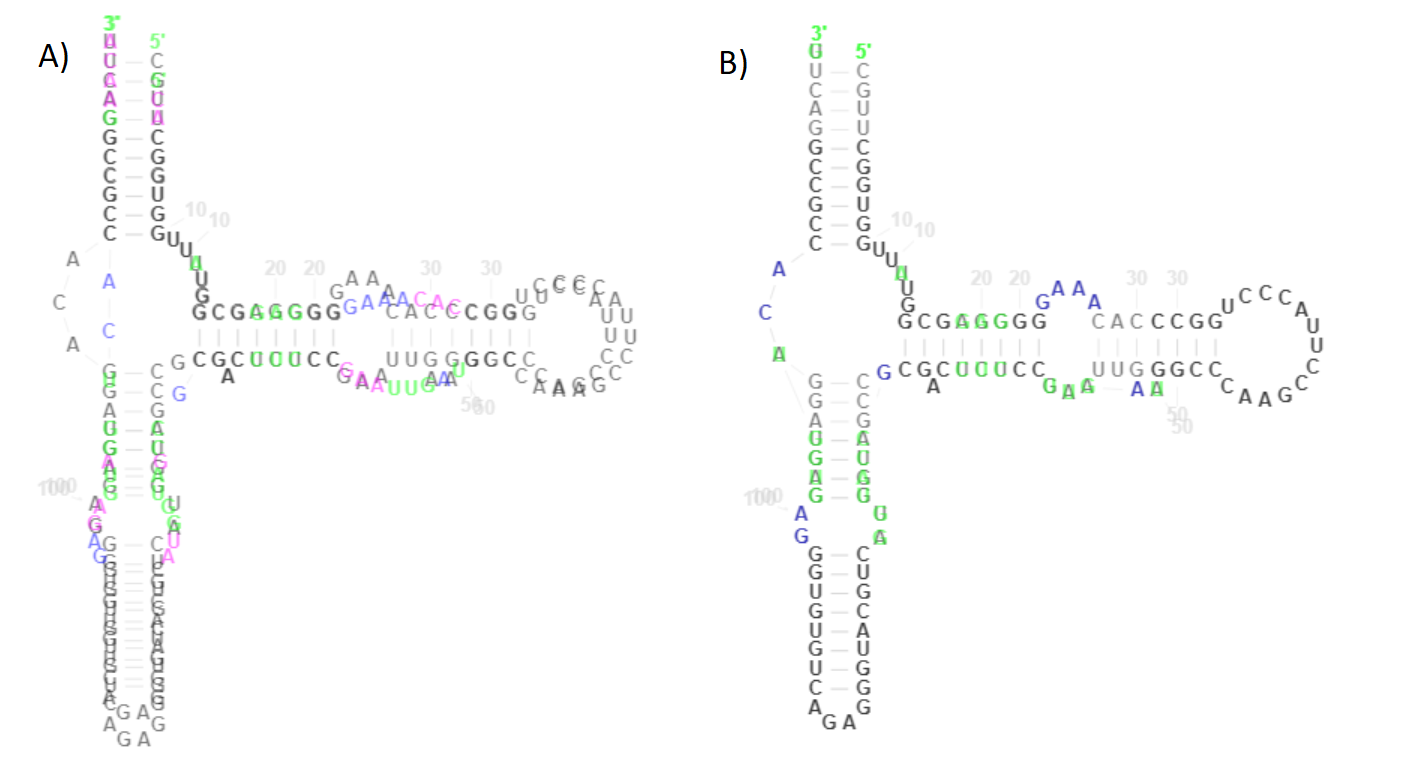
\includegraphics[width=140mm]{../img/kap02/animation.png}
  \caption{Vzorová a odvozená struktura přeložené přes sebe před transformací
  (A) a po transformaci (B).}
\end{figure}

\section{Mapovací čáry}

Vědomost o tom, který nukleotid se na co mapuje, může být významná pro odhalení
rozdílů a podobností mezi strukturami. V našem úsilí zprostředkovat tuto
informaci již před transformací na vzorovou sturkturu jsme přišli s dalším
způsobem - s čárami, které spojují každý nukleotid s jeho vzorovým nukleotidem.

\begin{figure}[H]
  \centering
  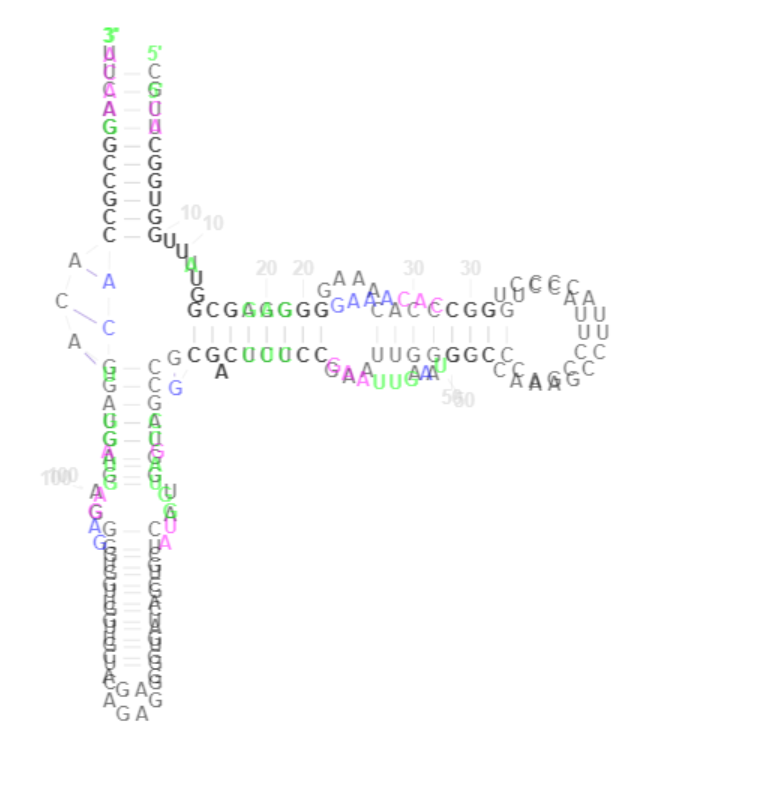
\includegraphics[height=90mm]{../img/kap02/mappingLines/small.png}
  \caption{Vzorová a odvozená struktura  přeložené přes sebe s mapovacíma
  čárama.}
\end{figure}

Bohužel tento způsob se zvětšující se velikostí struktury stáva velmi
nepřehledným, přesto si myslíme že můžou být užitečné a naše knihovna je
podporuje.

\begin{figure}[H]
  \centering
  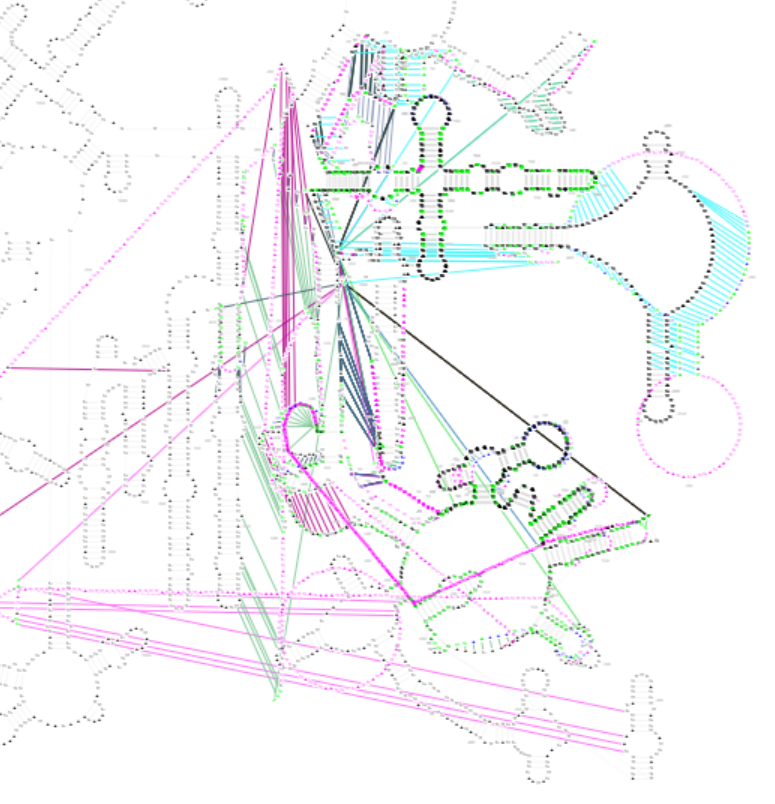
\includegraphics[width=140mm]{../img/kap02/mappingLines/big.png}
  \caption{Výřez z mnoha struktur přeložených přes sebe s mapovacími čárami.
  Každá struktura má vlastní barvu mapovacích čar.}
\end{figure}

\section{Demonstrace metod}

V rámci naší knihovny jsme vytvořili také webovou
aplikaci\footnote{https://michalhercik.github.io/rna-visualizer/}, která
demonstruje možnosti naší knihovny. Tato aplikace umožňuje uživatelům pracovat
s jednotlivými metodami pro usnadnění porovnání zmíněnými v této kapitole nebo
souběžně se všemi.
